\documentclass[]{article}

\usepackage{enumerate}
\usepackage{amssymb}
\usepackage{graphicx}

\def\OR{\vee}
\def\AND{\wedge}
\def\imp{\rightarrow}
\def\math#1{$#1$}
\def\mand#1{$$#1$$}
\def\mld#1{\begin{equation}
#1
\end{equation}}
\def\eqar#1{\begin{eqnarray}
#1
\end{eqnarray}}
\def\eqan#1{\begin{eqnarray*}
#1
\end{eqnarray*}}
\def\cl#1{{\cal #1}}

\DeclareSymbolFont{AMSb}{U}{msb}{m}{n}
\DeclareMathSymbol{\N}{\mathbin}{AMSb}{"4E}
\DeclareMathSymbol{\Z}{\mathbin}{AMSb}{"5A}
\DeclareMathSymbol{\R}{\mathbin}{AMSb}{"52}
\DeclareMathSymbol{\Q}{\mathbin}{AMSb}{"51}
\DeclareMathSymbol{\I}{\mathbin}{AMSb}{"49}
\DeclareMathSymbol{\C}{\mathbin}{AMSb}{"43}

\begin{document}
\bf \Large Gabriel Maayan - FOCS Assignment 2

\section{DMC 3.3}
Liamsi has more RAM than Kilam = p :  Pigs can fly = q

\math{\newline}p = T, q = F
\begin{enumerate}[(a)]
\item \math{\neg p\to q = T}
\item \math{p\to q = F}
\item \math{\neg p\land q = F}
\item \math{\neg p\lor q = F}
\item \math{p\land q = F}
\item \math{p\lor q = T}
\end{enumerate}•

\section{DMC 3.21}
\begin{enumerate}[(c)]
\item \math{\neg p\land q\land \neg r}
\end{enumerate}

\section{DMC 4.7}
\begin{enumerate}[(a)]
\item Prove "\math{x} is irrational \math{\to \sqrt{x}} is irrational."
\math{\\} Let \math{\sqrt{x}} be rational.
\math{\\ \sqrt{x} = a/b, a\in \Z , b\in \N
\\ x = {a^2}/{b^2}
\\ a^2/b^2} is rational. So x is rational.
\math{\\} $\therefore$ \math{x} is irrational \math{\to \sqrt{x}} is irrational, is True.

\end{enumerate}

\section{DMC 4.25 and 4.26}
\begin{enumerate}[(b)]
\item
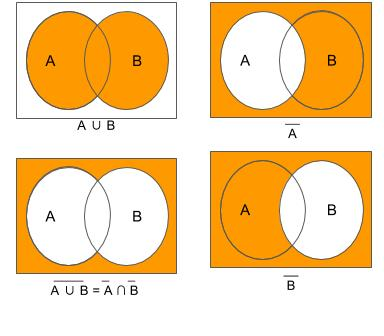
\includegraphics[width=\linewidth]{FOCSHW2}

\math{(A\cup B)'
\\} by DeMorgan's Thm
\math{\\ A' \cap B'
\\ \therefore (A\cup B)' = A' \cap B'}
\end{enumerate}

\section{DMC 4.13}
\begin{enumerate}[(l)]
\item Prove: If \math{x, y} are irrational, then $y^x$ is irrational.

Let \math{x = \log_{2} (9)} and \math{y = \sqrt{2}}
\math{\\ y^x = \sqrt{2}^{\log_{2} (9)}
\\ 2^{\log_{2} (3)}
\\ = 3
\\ \therefore} There can be an irrational \math{x, y} s.t. \math{y^x} is rational.

\end{enumerate}
\begin{enumerate}[(o)]
\item Prove \math{\exists x, y\in \Z : 2x^2+5y^2=14}

Let \math{y=0}, for \math{x = 0, 1, 2, 3, \cdots ,} \math{2x^2 = \{ 0, 2, 8, 18, \cdots \}\\}
Let \math{y=1}, for \math{x = 0, 1, 2, 3, \cdots ,} \math{2x^2 + 5 = \{ 5, 7, 13, 23, \cdots \}\\}
Let \math{y=2}, for \math{x = 0, 1, 2, 3, \cdots ,} \math{2x^2 + 20 = \{ 20, 22, 28, 38, \cdots \}\\
\therefore \exists x, y\in \Z : 2x^2+5y^2=14} is False.

\end{enumerate}•

\end{document}